\documentclass[11pt]{article}

% Change "review" to "final" to generate the final (sometimes called camera-ready) version.
% Change to "preprint" to generate a non-anonymous version with page numbers.
\usepackage[review]{acl}

% Standard package includes
\usepackage{times}
\usepackage{latexsym}

% For proper rendering and hyphenation of words containing Latin characters (including in bib files)
\usepackage[T1]{fontenc}
% For Vietnamese characters
% \usepackage[T5]{fontenc}
% See https://www.latex-project.org/help/documentation/encguide.pdf for other character sets

% This assumes your files are encoded as UTF8
\usepackage[utf8]{inputenc}

% This is not strictly necessary, and may be commented out,
% but it will improve the layout of the manuscript,
% and will typically save some space.
\usepackage{microtype}

% This is also not strictly necessary, and may be commented out.
% However, it will improve the aesthetics of text in
% the typewriter font.
\usepackage{inconsolata}

%Including images in your LaTeX document requires adding
%additional package(s)
\usepackage{graphicx}

% If the title and author information does not fit in the area allocated, uncomment the following
%
%\setlength\titlebox{<dim>}
%
% and set <dim> to something 5cm or larger.


% ADDITIONAL PACKAGES
\usepackage{booktabs}
\usepackage{tabularx}
\usepackage{array}
%

\title{Placeholder}

% Author information can be set in various styles:
% For several authors from the same institution:
% \author{Author 1 \and ... \and Author n \\
%         Address line \\ ... \\ Address line}
% if the names do not fit well on one line use
%         Author 1 \\ {\bf Author 2} \\ ... \\ {\bf Author n} \\
% For authors from different institutions:
% \author{Author 1 \\ Address line \\  ... \\ Address line
%         \And  ... \And
%         Author n \\ Address line \\ ... \\ Address line}
% To start a separate ``row'' of authors use \AND, as in
% \author{Author 1 \\ Address line \\  ... \\ Address line
%         \AND
%         Author 2 \\ Address line \\ ... \\ Address line \And
%         Author 3 \\ Address line \\ ... \\ Address line}

\author{First Author \\
  Affiliation / Address line 1 \\
  Affiliation / Address line 2 \\
  Affiliation / Address line 3 \\
  \texttt{email@domain} \\\And
  Second Author \\
  Affiliation / Address line 1 \\
  Affiliation / Address line 2 \\
  Affiliation / Address line 3 \\
  \texttt{email@domain} \\}

%\author{
%  \textbf{First Author\textsuperscript{1}},
%  \textbf{Second Author\textsuperscript{1,2}},
%  \textbf{Third T. Author\textsuperscript{1}},
%  \textbf{Fourth Author\textsuperscript{1}},
%\\
%  \textbf{Fifth Author\textsuperscript{1,2}},
%  \textbf{Sixth Author\textsuperscript{1}},
%  \textbf{Seventh Author\textsuperscript{1}},
%  \textbf{Eighth Author \textsuperscript{1,2,3,4}},
%\\
%  \textbf{Ninth Author\textsuperscript{1}},
%  \textbf{Tenth Author\textsuperscript{1}},
%  \textbf{Eleventh E. Author\textsuperscript{1,2,3,4,5}},
%  \textbf{Twelfth Author\textsuperscript{1}},
%\\
%  \textbf{Thirteenth Author\textsuperscript{3}},
%  \textbf{Fourteenth F. Author\textsuperscript{2,4}},
%  \textbf{Fifteenth Author\textsuperscript{1}},
%  \textbf{Sixteenth Author\textsuperscript{1}},
%\\
%  \textbf{Seventeenth S. Author\textsuperscript{4,5}},
%  \textbf{Eighteenth Author\textsuperscript{3,4}},
%  \textbf{Nineteenth N. Author\textsuperscript{2,5}},
%  \textbf{Twentieth Author\textsuperscript{1}}
%\\
%\\
%  \textsuperscript{1}Affiliation 1,
%  \textsuperscript{2}Affiliation 2,
%  \textsuperscript{3}Affiliation 3,
%  \textsuperscript{4}Affiliation 4,
%  \textsuperscript{5}Affiliation 5
%\\
%  \small{
%    \textbf{Correspondence:} \href{mailto:email@domain}{email@domain}
%  }
%}

\begin{document}
\maketitle
\begin{abstract}
% Word count: 181
The emergence of Large Audio Language Models (LALMs) has broadened access to advanced and currently developing language technologies by supporting audio input alongside text. However, this convenience has primarily benefited speakers of high-resource languages, when this can be valuable to speakers of languages in low-resource settings, especially those where speech is the primary mode of communication. While recent research has focused on including low-resource languages by simply restricting training to a linear projector connecting a speech encoder and a large language model, as the decoder, the impact of the specialization of the large language model (LLM) used as the decoder remains unexplored in this setup. In this work, we investigate decoder specialization using a family of state-of-the-art (SOTA) small multilingual LLMs developed specifically to address the challenges of low-resource languages.

Extensive experiments across 12 languages, spanning a range of resource levels, including morphologically rich languages that remain challenging for automatic speech recognition (ASR) systems, reveal only minor differences in character error rate (CER) between the three regionally specialized decoders and their general-purpose counterpart. We release all checkpoints to support further investigation.

\end{abstract}

\section{Introduction}

Automatic speech recognition (ASR) models such as Whisper \citep{radfordRobustSpeechRecognition} and Omnilingual ASR\citep{teamOmnilingualASROpenSource2025} have expanded multilingual speech recognition to a growing number of languages, including low-resource languages. Despite this progress, substantial work remains to address the breadth and diversity of low resource languages and dialects, which has motivated recent studies to investigate the failure modes of these systems in low-resource settings \citep{imamAutomaticSpeechRecognition, kyslyiBuildingASRResources, kumarOvercomingDecoderInconsistencies2026, bharathiFindingsTamilDialect, azisDevelopmentLowResourceAutomatic2026}.  These limitations are important to address because language technologies today are increasingly multimodal, although text-based interfaces as the default in many settings and the speech modality is still developed primarily for high-resource languages. This is crucial given that, of the roughly 7,000 languages spoken worldwide, around 4,000 are estimated to
have an established writing system, however, it does not correspond to widespread literacy or everyday use among speakers \footnote{Ethnologue, 28th edition \url{https://www.ethnologue.com/}}. Considering this, Speech-first technologies may benefit speakers of languages in low resource settings by enabling them access to services that are better supported in high resource languages with current technologies. However developing end-to-end speech language systems remains computationally expensive and relies on abundant, high-quality annotated data. 

One recent direction addressing these constraints is the SLAM-ASR architecture \citep{maEmbarrassinglySimpleApproach2024}, which connects a pretrained speech encoder to a large language model (LLM) through a trainable linear projector, while keeping the pretrained models frozen.  Restricting training to the projector provides a practical way to introduce a language in low-resource settings. Studies building on this work have investigated its robustness \citep{kumarPerformanceEvaluationSLAMASR2025}, number of necessary audio hours \citep{fongSpeechLLMsLowResource2025}, which encoder layers can be pruned while maintaining performance through fine-tuning of the LLM backbone \citep{kolluriRoleEncoderDepth2026}, language-level and language-family-level training configurations \citep{zhangLanguageFamilyMatters2026}, and reducing prompt sensitivity with a learnable prompt projector \citep{burdissoReducingPromptSensitivity2026}. Although these prior studies have investigated several aspects of SLAM-ASR, the decoder selection has generally been guided by target-language support and state-of-the-art (SOTA) multilingual coverage, [TODO: Add Examples of the LLMs they used]. To the best of our knowledge, however, the effect of decoder specialization within this architecture has not been systematically evaluated, leaving open whether specialized decoders provide an advantage over general-purpose models unexplored. More recently, the Tiny Aya family\citep{salamancaTinyAyaBridging2026} introduced SOTA small multilingual LLMs that share a common multilingual foundation, with each regional model having undergone post-training to reinforce the linguistic clusters associated with its respective region. 

% Tried framing this for negative results
Motivated by the growing study of failure modes in low-resource ASR and recent advances in small regionally specialized multilingual LLMs, we aim to contribute to the efforts to build linguistically informed language technologies. In this study we address the unexplored role of decoder specialization within the SLAM-ASR architecture by examining empirically comparing regional Tiny Aya decoders wth Tiny Aya Global across 10 languages , [TODO: Update]nine  are from the three Tiny Aya regional clusters and one language unsupported by both and % REVIEW: this says 10 languages; the study covers 12 (11 with a Tiny Aya region, plus
% Kreol Seselwa, which has none). The abstract already says 12.
examining whether and to what extent specialization offers a strong starting point for low-resource languages when ASR data are scarce. [TODO: Introduce research questions(s) ?]



% ADDED (first draft): positions SLAM-ASR as a low-resource route and states the language
% coverage contribution. Placed here rather than in a new \section{Related Work} so the existing
% structure is untouched; promote it to its own section in a later pass if preferred.
\paragraph{SLAM-ASR as a route into low-resource languages.}
The appeal of this architecture for low-resource settings is that almost nothing has to be
trained. The encoder and the decoder are frozen and can be taken off the shelf, and the only
optimized component is a projector of a few million parameters, so a language can be added with
a few hours of transcribed audio and a single GPU rather than with a full ASR training pipeline.
\citet{fongSpeechLLMsLowResource2025} quantify where that route becomes competitive, finding
that roughly 100--200 hours are needed before the framework matches a Whisper-only baseline, and
that projector pretraining on a high-resource language substantially improves the low-resource
end. Reviews of African ASR report the same shortage from the data side
\citep{imamAutomaticSpeechRecognitionAfrican2025, adjoviSpeechTextCorpora2026}.

Most SLAM-ASR studies to date evaluate on a small set of well-resourced languages. Of the twelve
languages we study, seven --- French, Marathi, Urdu, Swahili, Hausa, Amharic and Kreol Seselwa
--- are not examined in the speech-LLM literature we survey, and Kreol Seselwa appears not to
have been evaluated in this architecture at all. Reporting them together, under one recipe and
one encoder, is part of what this study contributes.

\section{Methods}
\subsection{SLAM-ASR}

\begin{figure}[t]
  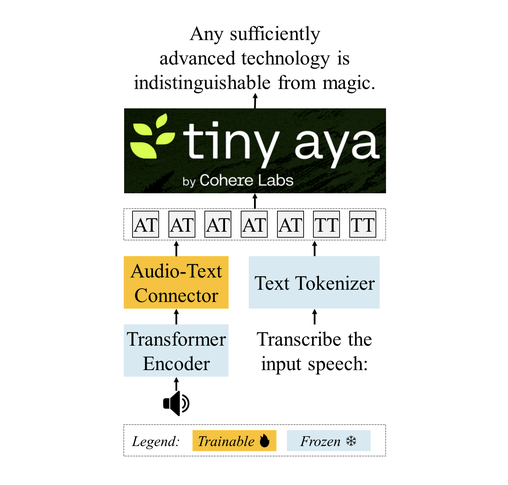
\includegraphics[width=\columnwidth]{assets/images/ph_listaya.png}
  \caption{LisTAya}
  \label{fig:ph_listaya}
\end{figure}


%Note: Cover the trainable linear projector

[TODO:  then remove specifics of encoder and decoder names and write them at the end. ]
Our implementation follows the Encoder--Connector--Decoder architecture introduced in SLAM-ASR \citet{maEmbarrassinglySimpleApproach2024} and is built upon the Qwen2-Audio codebase \footnote{Qwen2-Audio codebase, \url{Qwen2-Audio codebase}}, as Illustrated in Figure~\ref{fig:ph_listaya}
%which follows an Encoder--Connector (projector)--Decoder framework. A frozen encoder first extracts acoustic representations from the input speech. These representations are then downsampled and projected into the embedding space through a trainable  Connector (projector). The projected speech embeddings are subsequently provided to the frozen  decoder, which autoregressively generates the transcription.

Following the original SLAM-ASR framework, only the Connector (projector) is optimized during training, while both the  encoder and the  decoder remain frozen. This design enables efficient adaptation by learning the alignment between speech representations and the language model embedding space while minimizing the number of trainable parameters.  

\subsection{Decoder Specialization}
PH Note: Add details regarding the Tiny Aya Family, include a table.

To study the effect of decoder specialization on multilingual ASR, we employ models from the \textit{TinyAya} family as the frozen decoder within the SLAM-ASR architecture. 


\textit{TinyAya-Base} is a pretrained 3.35B-parameter multilingual language model covering more than 70 languages. Built upon this foundation, \textit{TinyAya-Global} provides balanced instruction-tuned performance across 67 languages, while three regionally specialized variants are available: \textit{TinyAya-Earth} for languages from Africa and West Asia, \textit{TinyAya-Fire} for South Asian languages, and \textit{TinyAya-Water} for languages from the Asia-Pacific and Europe.

[TODO: Post training for each variant, tokenizer specialization]

All TinyAya variants share a common multilingual tokenizer, which is trained using a balanced weighting strategy that combines data-distribution and language-family information to achieve equitable representation of both high- and low-resource languages. Furthermore, TinyAya adopts a region-aware multilingual posttraining strategy in which high-quality instruction-tuning data is constructed through language-specific translation, prompt transformation, and Fusion-of-N teacher generation, enabling balanced multilingual instruction tuning across diverse language groups while improving coverage for low-resource languages.

%Across all experiments, the Whisper speech encoder and the trainable Connector (projector) remain unchanged, while only the frozen \textit{TinyAya} decoder is replaced with a different variant. This controlled setup isolates the effect of decoder specialization on multilingual ASR while keeping all other architectural components and training procedures identical.


\section{Experimental Setup}
\subsection{Datasets}
Our experiments use two multilingual speech corpora: World Speech \citep{asonitisWorldSpeechMultilingualSpeech2026} and FLEURS\citep{conneauFLEURSFEWShotLearning2023}. WorldSpeech primarily contains formal speech collected from diverse public sources such as parliamentary proceedings, international broadcasts, with smaller contributions from public-domain audiobooks. FLEURS contains read speech based on parallel sentences from the FLoRes-101 dataset, recorded were under relatively controlled conditions. We use subsets of train sets from WorldSpeech for training, excluding audio samples with durations of 30 seconds or longer. For evaluation, we use the validation sets from FLEURS when available and on the WorldSpeech test sets otherwise. 

We select 12 languages for this study (Table~\ref{tab:dataset-overview}). 11 are covered by the regional Tiny Aya models:  Water (English, French, Spanish, and Indonesian), Fire (Hindi, Tamil, Marathi, and Urdu), and Earth (Swahili, Hausa, Amharic). Kreol Seselwa is an African language selected because it is unsupported by both backbone models. We include it to assess whether the trainable connector (projector) can effectively learn the alignment between speech representations and the language model, despite this lack of support.


%These datasets provide diverse multilingual speech samples for evaluating the effectiveness of different TinyAya decoder variants.

%From the \textit{TinyAya-Water} region, we include English, French, Spanish, and Indonesian. From \textit{TinyAya-Fire}, we select Hindi, Tamil, and Marathi, while Swahili and Hausa are chosen from \textit{TinyAya-Earth}. These 9 languages are supported by both the Whisper encoder and the corresponding TinyAya decoder variants.



\subsection{Training Configuration}
%[TODO Find other info in WandB]

In our study, we use \textbf{Lis}tening \textbf{T}iny \textbf{A}ya (LisTAya; see Figure~\ref{fig:ph_listaya}) to refer to models that use Whisper Medium as the fixed speech encoder, paired with different regional variants from the Tiny Aya family as decoders. Depending on the specialized regional decoder we refer to the resulting models as LisTAya-Water, LisTAya-Fire, LisTAya-Earth; LisTAya-Global for the general-purpose variant.

Throughout all experiments, we train only the projector while keeping the encoder and decoder components frozen. We use the AdamW optimizer with a learning rate set at 1.5e-3, training steps 1, 000, batch size 8, gradient accumulation of 64 (an effective batch size of 512), and no weight decay. We retain the checkpoint after 1,000 steps, as well as an additional checkpoint achieving the lowest validation CER. All models were trained with one NVIDIA H200 GPU.


\begin{table}[t]
\centering

\setlength{\tabcolsep}{5pt}
\renewcommand{\arraystretch}{1.08}

\begin{tabular}{@{}lll@{}}
\toprule
& \textbf{WorldSpeech} & \textbf{FLEURS} \\
\cmidrule(lr){2-2} \cmidrule(l){3-3}

\textbf{Language} & \textbf{Train} & \textbf{Test} \\
\midrule
English & en\_us & en\_us   \\
Spanish & es\_mx & es\_419  \\
French & fr\_ca & fr\_fr   \\
% REVIEW: manifest_training.csv records the Indonesian training config as id_id, not in_in.
Indonesian & in\_in & id\_id  \\
\midrule
Hindi & hi\_in & hi\_in   \\
Marathi & mr\_in & mr\_in   \\
% REVIEW: Tamil trains on ta_in alone. Verified over the full config: all 23,261 ta_lk clips
% are exactly 30.00 s and the strict < 30 s filter removes every one, so ta_lk never reached
% the model. The W&B configs have been corrected accordingly.
Tamil & ta\_in & ta\_in   \\
% REVIEW: the training config lists ur_pk first, then ur_in.
Urdu & ur\_in $+$ ur\_pk & ur\_pk   \\
\midrule
Swahili & sw\_ke $+$ sw\_tz & sw\_ke   \\
% REVIEW: manifest_training.csv records the Amharic training config as am_et, not am_te.
Amharic & am\_te & am\_et   \\
Hausa & ha\_ng $+$ ha\_td  & \textbf{ha\_ng}  \\
Kreol Seselwa & crs\_sc & \textbf{crs\_sc} \\

\bottomrule
\end{tabular}

% REVIEW: tables/tab_datasets.tex is generated from data/manifest_training.csv and carries
% resource tier and evaluation-set size. Consider replacing this hand-written body with
% % GENERATED by build_paper_tables.py -- edit that script, not this file.
\begin{table}[t]
\centering
\setlength{\tabcolsep}{4pt}
\begin{tabular}{@{}llrr@{}}
\toprule
\textbf{Language} & \textbf{WorldSpeech train} & \textbf{Tier} & \textbf{Eval $n$} \\
\midrule
English & en\_us & high & 35336 \\
Spanish (LatAm) & es\_mx & high & 10839 \\
French & fr\_ca & high & 10919 \\
Indonesian & id\_id & high & 5323 \\
\midrule
Hindi & hi\_in & high & 27474 \\
Marathi & mr\_in & mid & 3064 \\
Tamil & ta\_in & very low & 466 \\
Urdu & ur\_pk $+$ ur\_in & low & 1482 \\
\midrule
Amharic & am\_et & very low & 468 \\
Hausa & ha\_ng $+$ ha\_td & mid & 810 \\
Swahili & sw\_ke $+$ sw\_tz & high & 5352 \\
\midrule
Seychellois Creole & crs\_sc & high & 19162 \\
\bottomrule
\end{tabular}
\caption{Training configuration and evaluation-set size per language, generated from the run manifest.}
\label{tab:dataset-generated}
\end{table}
 in a later pass.
\caption{Dataset overview. WorldSpeech training subsets are used to train the
projector. Evaluation uses the FLEURS validation split; bold entries use the
WorldSpeech test split. The \(+\) symbol denotes subsets pooled.}

%and language subsets used for training and evaluation.


\label{tab:dataset-overview}
\end{table}



\section{Results}

% ADDED (first draft). Numbers come from tables/*.tex, generated by build_paper_tables.py in
% the analysis repo, so nothing here is transcribed by hand.

\subsection{Decoder specialization does not change what the model hears}

Table~\ref{tab:region-match} reports, for each language, the best CER of the region-matched
decoder against the mean of the two mismatched regional decoders and against LisTAya-Global.
Across the 11 languages covered by a Tiny Aya region, the matched decoder is
\textbf{0.55 CER better} on average, with a 95\% confidence interval of $[-3.89, 1.99]$ and a
Wilcoxon signed-rank $p = 0.966$. Six of eleven languages favour the matched decoder and five do
not.

This is a null, and its width is what makes it informative. The paired design's minimum
detectable effect is \textbf{4.90 CER}, so effects smaller than that cannot be resolved here.
We also measure the run-to-run floor directly rather than assuming it: over ten replicate pairs
in which a cell was trained twice, the between-run standard deviation is \textbf{1.17 CER},
against a median within-run late-training standard deviation of 1.09. The observed effect is
smaller than the noise between two runs of the same configuration.

% GENERATED by build_paper_tables.py -- edit that script, not this file.
\begin{table*}[t]
\centering
\setlength{\tabcolsep}{4pt}
\begin{tabular}{@{}llrrrr@{}}
\toprule
\textbf{Language} & \textbf{Region} & \textbf{Match} & \textbf{Mism.} & \textbf{Global} & \textbf{$\Delta$} \\
\midrule
Amharic & Earth & 29.25 & 27.93 & 27.00 & 1.32 \\
Tamil & Fire & 43.63 & 58.33 & 61.21 & -14.70 \\
Urdu & Fire & 22.24 & 20.81 & 17.64 & 1.44 \\
Hausa & Earth & 33.43 & 34.62 & 35.03 & -1.19 \\
Marathi & Fire & 13.57 & 14.01 & 14.14 & -0.44 \\
English & Water & 12.05 & 4.67 & 4.96 & 7.39 \\
Spanish (LatAm) & Water & 3.41 & 3.35 & 3.40 & 0.07 \\
French & Water & 6.36 & 6.79 & 6.61 & -0.43 \\
Hindi & Fire & 13.11 & 12.05 & 13.18 & 1.06 \\
Indonesian & Water & 5.74 & 6.14 & 6.05 & -0.40 \\
Swahili & Earth & 13.53 & 13.68 & 12.60 & -0.15 \\
\bottomrule
\end{tabular}
\caption{Best CER per language for the region-matched decoder, the mean of the two mismatched regional decoders, and LisTAya-Global. $\Delta$ is matched minus mismatched; negative favours the matched decoder. Ordered by resource tier.}
\label{tab:region-match}
\end{table*}


\subsection{The specialization is small in the data}

A null invites the question of whether the manipulation was large enough to detect. We quantify
it from the Tiny Aya report's own language-composition tables: for each language we take the
share of the matched variant's post-training mix in that language, minus the mean share of the
two mismatched variants. The median excess is \textbf{1.3 percentage points}.

Regional specialization in this model family is therefore a shift of about one percentage point
of post-training data per language, not a change of training corpus. Read against that, the
result is better stated as \emph{specialization at this magnitude does not measurably change
recognition accuracy}, which is a narrower and more useful claim than specialization being
inert.

\subsection{Training data volume predicts overfitting}

While decoder choice does not predict accuracy, the amount of training audio predicts how a run
behaves. Table~\ref{tab:loss-tier} groups languages by resource tier and reports the rise in
evaluation loss after its own minimum, and the fraction of the run elapsed at that minimum. Both
are monotone across the four tiers: the lowest-resource cells reach their best evaluation loss
about a quarter of the way through training and degrade over the remaining three quarters, while
the highest-resource cells improve almost to the end.

% GENERATED by build_paper_tables.py -- edit that script, not this file.
\begin{table}[t]
\centering
\setlength{\tabcolsep}{4pt}
\begin{tabular}{@{}lrrr@{}}
\toprule
\textbf{Tier} & \textbf{Langs} & \textbf{Eval-loss rise} & \textbf{Frac.\ to best} \\
\midrule
very low & 2 & 0.211 & 0.282 \\
low & 1 & 0.188 & 0.292 \\
mid & 2 & 0.041 & 0.627 \\
high & 7 & 0.003 & 0.816 \\
\bottomrule
\end{tabular}
\caption{Overfitting by resource tier. Both columns are medians of per-language medians, so a tier with seven languages cannot outweigh one with two.}
\label{tab:loss-tier}
\end{table}


\subsection{Connector training versus off-the-shelf models}

Table~\ref{tab:baselines} compares each trained LisTAya checkpoint against the strongest
off-the-shelf model we evaluate on the same test set. In every cell evaluated so far, training a
projector on a few hours of in-language audio beats the best downloadable model, and the margin
is largest exactly where the baseline is weakest.

% TODO(first draft): this sweep is still running -- 4 of 43 cells at the time of writing.
% Re-run build_paper_tables.py before submission and update the sentence above with the final
% coverage.

% GENERATED by build_paper_tables.py -- edit that script, not this file.
\begin{table*}[t]
\centering
\setlength{\tabcolsep}{4pt}
\begin{tabular}{@{}lllrrr@{}}
\toprule
\textbf{Language} & \textbf{Test set} & \textbf{Domain} & \textbf{Base.} & \textbf{LisTAya} & \textbf{$\Delta$} \\
\midrule
Amharic & am\_et & FLEURS & 111.61 & 32.87 & -78.74 \\
Amharic & am\_et & in-domain & 133.07 & 30.45 & -102.62 \\
Seychellois Creole & crs\_sc & in-domain & 85.18 & 16.41 & -68.77 \\
English & en\_us & FLEURS & 2.11 & 5.54 & 3.43 \\
English & en\_au & in-domain & 9.46 & 14.93 & 5.47 \\
English & en\_jm & in-domain & 7.62 & 9.54 & 1.92 \\
English & en\_ke & in-domain & 19.49 & 23.81 & 4.32 \\
English & en\_nz & in-domain & 8.47 & 17.30 & 8.83 \\
English & en\_pk & in-domain & 78.47 & 422.88 & 344.41 \\
English & en\_sl & in-domain & 14.12 & 20.25 & 6.13 \\
English & en\_us & in-domain & 9.95 & 9.44 & -0.51 \\
English & en\_zm & in-domain & 15.83 & 21.38 & 5.55 \\
Spanish (LatAm) & es\_419 & FLEURS & 1.34 & 3.14 & 1.80 \\
Spanish (LatAm) & es\_ar & in-domain & 20.01 & 21.96 & 1.95 \\
Spanish (LatAm) & es\_cl & in-domain & 19.59 & 23.07 & 3.48 \\
Spanish (LatAm) & es\_co & in-domain & 11.79 & 15.16 & 3.37 \\
Spanish (LatAm) & es\_es & in-domain & 7.43 & 13.01 & 5.58 \\
Spanish (LatAm) & es\_mx & in-domain & 8.46 & 8.91 & 0.45 \\
Spanish (LatAm) & es\_pe & in-domain & 6.55 & 10.39 & 3.84 \\
Spanish (LatAm) & es\_pr & in-domain & 9.54 & 12.24 & 2.70 \\
Spanish (LatAm) & es\_py & in-domain & 8.65 & 12.36 & 3.71 \\
Spanish (LatAm) & es\_uy & in-domain & 20.69 & 23.48 & 2.79 \\
French & fr\_fr & FLEURS & 2.10 & 7.47 & 5.37 \\
French & fr\_ca & in-domain & 10.93 & 8.58 & -2.35 \\
French & fr\_cd & in-domain & 7.18 & 10.92 & 3.74 \\
French & fr\_ci & in-domain & 7.77 & 13.21 & 5.44 \\
Hausa & ha\_ng & FLEURS & 55.94 & 39.14 & -16.80 \\
Hausa & ha\_td & in-domain & 82.00 & 36.58 & -45.42 \\
Hindi & hi\_in & FLEURS & 5.74 & 13.73 & 7.99 \\
Hindi & hi\_in & in-domain & 24.50 & 25.75 & 1.25 \\
Indonesian & id\_id & FLEURS & 3.26 & 5.86 & 2.60 \\
Indonesian & id\_id & in-domain & 13.89 & 10.85 & -3.04 \\
Marathi & mr\_in & FLEURS & 19.45 & 14.39 & -5.06 \\
Marathi & mr\_in & in-domain & 18.62 & 10.36 & -8.26 \\
Swahili & sw\_ke & FLEURS & 26.32 & 15.10 & -11.22 \\
Swahili & sw\_ke & in-domain & 18.63 & 14.52 & -4.11 \\
Swahili & sw\_tz & in-domain & 45.45 & 13.46 & -31.99 \\
Tamil & ta\_in & FLEURS & 16.22 & 48.29 & 32.07 \\
Tamil & ta\_in & in-domain & 18.44 & 15.42 & -3.02 \\
Tamil & ta\_lk & in-domain & 64.30 & 69.06 & 4.76 \\
Urdu & ur\_pk & FLEURS & 11.65 & 20.04 & 8.39 \\
Urdu & ur\_in & in-domain & 20.17 & 17.35 & -2.82 \\
Urdu & ur\_pk & in-domain & 46.03 & 74.13 & 28.10 \\
\bottomrule
\end{tabular}
\caption{CER of the best off-the-shelf baseline against the best LisTAya checkpoint on the same test set. Negative $\Delta$ favours the trained projector.}
\label{tab:baselines}
\end{table*}


\subsection{A language neither component supports}

Kreol Seselwa is supported by neither the Whisper encoder nor any Tiny Aya decoder, and it is
the one cell where both frozen components operate outside their coverage. The four decoders span
17.92--21.35 CER on it, a range of 3.43 CER. The projector therefore learns a usable alignment
for a language absent from both pretraining corpora, and which regional variant it is paired
with matters as little there as elsewhere.



\section*{Limitations}

% ADDED (first draft).

Most cells are trained once. Ten of the 52 runs have a replicate, which is what lets us state a
between-run standard deviation of 1.17 CER, but the remaining cells carry no direct uncertainty
estimate, and the design's minimum detectable effect of 4.90 CER is well above the effects that
would be practically interesting. A negative result at this width bounds the effect rather than
excluding it.

Ten of the twelve languages train on WorldSpeech and evaluate on FLEURS, so most reported numbers
combine decoder choice with a domain shift from formal recorded speech to read speech. We report
in-domain WorldSpeech test results alongside them where available, but the two are not
separable in every cell.

The study measures transcription accuracy only. Whether decoder specialization affects
downstream spoken-language understanding, where the decoder's own multilingual knowledge is more
directly exercised, is not addressed here.

Finally, the comparison assumes the Tiny Aya variants differ only in post-training data. We take
that from the model family's own documentation rather than verifying it independently.


\section*{Acknowledgments}

PH

% Bibliography entries for the entire Anthology, followed by custom entries
%\bibliography{custom,anthology-overleaf-1,anthology-overleaf-2}

% Custom bibliography entries only
%\bibliography{LisTAya}
\bibliography{LisTAya_updated}
\appendix

\section{Example Appendix}
\label{sec:appendix}

This is an appendix.

\end{document}
